\chapter{環境識別子による型システムの構築}
プログラム実行時にエラーを起こさないようにしたい場合,
プログラムを動的に動かしてエラーを発見するのではなく,
静的にプログラムを解析し,意図したプログラムのみ実行できるようにする必要がある.
それを実現するひとつの方法として型システムを構築する方法がある.
以下の節では,コード生成体系にshift0/reset0 を導入した我々の体系に対して,安全なプログラムに対しては型が付き,それ以外の安全でないプログラムには型が付かないような型システム構築のアイデアを記す.

\section{先行研究のアイディア}
表現力と安全性を兼ね備えたコード生成の体系としては,2009年のKameyamaらの研究\cite{Kameyama2009}が最初である.彼ら は,MetaOCaml において shift/reset とよばれるコントロールオペレータを使うスタイルでのプログラミング を提案するとともに,コントロールオペレータの影響が変数スコープを越えることを制限する型システムを構築し,安全性を厳密に保証した.

Tahaら\cite{Taha:2003:EC:604131.604134}は,純粋な(副作用のない)コード生成の言語の型安全性を保証するため,
環境識別子(Environment Classifier)を導入した.
環境識別子$\alpha$は,コード生成のステージに対応し,
「そのステージで使える(コードレベル)の変数とその型の集合(あるいは型文脈)」を抽象的に表現した変
数であり,$\codeT{\intT}{\alpha}$のように,コード型の一部として使用される.

須藤ら\cite{Sudo2014}は,破壊的変数を持つコード生成言語に対する型安全性を保証するため,
環境識別子を精密化した.本節では,須藤らのアイディアを解説する.
以下の図は,彼らの言語における危険なプログラム例である.

\begin{figure}[ht]
  \centering
  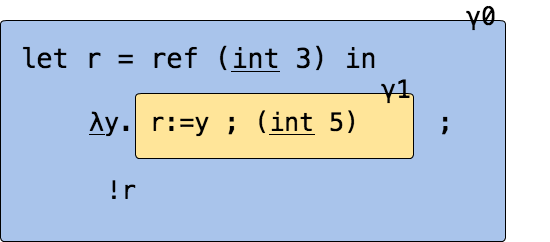
\includegraphics[clip,width=10cm]{./img/sudo_ref.png}
  \caption{危険な例}
  \label{fig:sudo_ref}
\end{figure}


ここで,$r$は,整数のコードを格納する参照(破壊的セル)であり,$r:=y$と
$!r$はそれぞれ,$r$への代入と$r$の中身の読み出しを表す.
上記のプログラムは,コードレベルのラムダ抽象($y$に対するラムダ抽象)で
生成されるコードレベル変数を$u$とするとき,$\code{u}$を$r$に格納し,
$u$のスコープ(黄色で示したもの)が終わったあとに取り出しているため,
計算結果は,自由変数をもつコード$\code{u}$となり,危険である.

上記のようなプログラムを型エラーとするため,須藤らは,コードレベル変数の
スコープごとに環境識別子を割り当てた.
上記では外側のスコープ(青)が$\gamma_0$,
内側のスコープ(黄)が$\gamma_1$という環境識別子で表現される.
$\gamma_0$で有効なコードレベル変数はなく,
$\gamma_1$で有効なコードレベル変数は$y$(に対応して生成される変数)である.
$\gamma_0$のスコープは$\gamma_1$のスコープを含む.言い換えれば,
$\gamma_1$で使える変数の方が$\gamma_0$で使える変数の方が(同じか)多い.
このことを$\gamma_1 \ord \gamma_0$ と表すことにする.
$r$は $\codeT{\intT}{\gamma_0} \mbox{\texttt{ref}}$型を持つ.
$y$は $\gamma_1$で使える変数であるが,$\gamma_0$では使えないため,
$r$に$y$を代入することはできず,$r:=y$のところで型エラーとなる.

コードレベルの変数スコープと,型によるスコープの表現をあらわしたのが,以下の図である.
forやletなどコードレベルの束縛子があるたびに,新しいスコープが開かれ,
使える変数が増えていくことが分かるだろう.

\begin{figure}[ht]
  \centering
  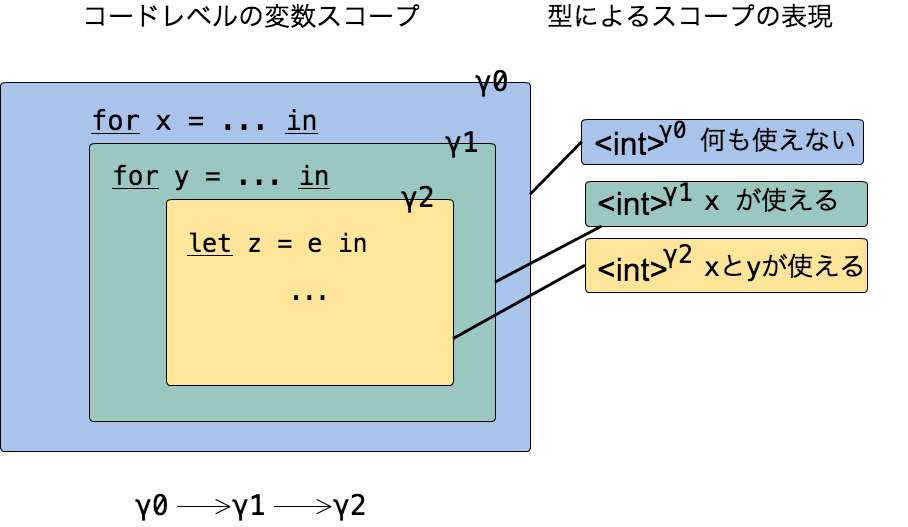
\includegraphics[clip,height=8cm]{./img/ec_for.png}
  \caption{型によるコードレベル変数のスコープ表現}
  \label{fig:ec_for}
\end{figure}

コードレベルの変数の型に,(精密化した)環境識別子を付与することで,その
変数が使えるスコープがわかり,破壊的代入などの副作用があるプログラムにおいても
スコープや型の安全性を保つことができる.

なお,須藤らの対象としていた言語が持っていた計算エフェクトは,「局所的なスコープをもつ参照」
であり,現実のOCaml/MetaOCaml等とは異なるものであった.
同一の著者グループは,最近,精密化した環境識別子のアイディアを用いて,
グローバルな参照を持つ言語に対するある種の型安全性
が成立することを示している\cite{Aplas2016}.

\section{本研究: 環境識別子の拡張}

本研究で扱う shift0/reset0によるコントロールエフェクトは,
須藤らによる精密化された環境識別子でも扱うことができない.本節では,そ
の問題点を明らかにし,その問題の解決の鍵となる join ($\cup$)の導入につ
いて述べる.

このため,前述の2重のforループ生成において,その中間にlet挿入をするプログラムに
ついて考察する.その概形は\ref{fig:ecex_for_non_gamma}図の上図である.

\begin{figure}[H]
  \centering
  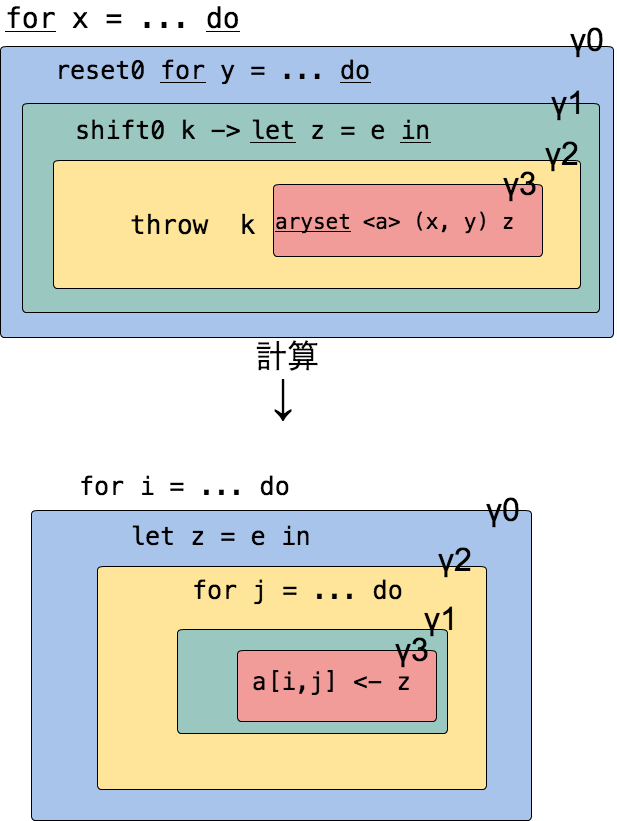
\includegraphics[clip,height=12cm]{./img/ecex_for_non_gamma.png}
  \caption{コード生成によるlet挿入}
  \label{fig:ecex_for_non_gamma}
\end{figure}

\ref{fig:ecex_for_non_gamma}図で,使えるコードレベル変数が異なる場所ごとに,
$\gamma_0,\gamma_1,\gamma_2,\gamma_3$と名付けた.
須藤らの体系通りであれば,これらの環境識別子の間の順序は,スコープの包
含関係通りであるので,

\begin{figure}[H]
  \centering
  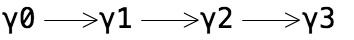
\includegraphics[clip,width=4cm]{./img/gamma_normal.png}
  \caption{誤った環境識別子の順序}
  \label{fig:gamma_normal}
\end{figure}

\ref{fig:gamma_normal}図のような順序がつくはずである.
しかし,計算を進めて得られたコード(\ref{fig:ecex_for_non_gamma}図の下図)を見ると,
$\gamma_1$(緑色)と$\gamma_2$(黄色)の位置関係が入れ代わっている.
結果のコードの型が整合する(束縛変数が自由になることはない等)ために
は,$\gamma_2$において$\gamma_1$で使える変数を使ってはいけないことがわかる.
一方で,赤字で示された$\gamma_3$においては,$\gamma_1$の変数も
$\gamma_2$の変数も使って構わない.
これらを考慮すると,環境識別子の間の順序は\ref{fig:gamma}図となる.

\begin{figure}[H]
  \centering
  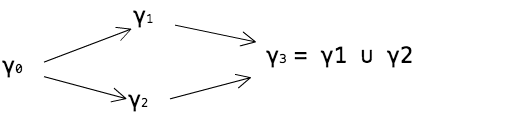
\includegraphics[clip,width=7cm]{./img/gamma.png}
  \caption{正しい環境識別子の順序}
  \label{fig:gamma}
\end{figure}

ここでのポイントは,$\gamma_0$ から,2つの異なる(包含関係のな
い)$\gamma_1$と$\gamma_2$に別れたあと,再び$\gamma_3$で合流することで
ある.須藤らの体系では,環境識別子のなす半順序集合全体は木の形であったが,
本研究の体系では,このように1度別れたものが合流することがある.
なお,$\gamma_3$で使える変数の集合は$\gamma_1$と$\gamma_2$で使える変数の和集
合と一致するので$\gamma_3 = \gamma_1 \cup \gamma_2$とおくことができる.
このように,環境識別子の世界に Join ($\cup$)を導入することによ
り,コントロールオペレータによる文脈の移動に対応できることになった.

\section{本研究: 型システムの構築}

本研究の基本アイディアは前項で述べたようなシンプルなものであるが,
言語体系と型システムの構築にあたってはいくつかの困難があった.
ここでは,そのうち,コントロールオペレータが切りとった継続に関する多相性について述べる.

前節の例では,shift0 が切り取る文脈(継続)は,
穴が$\gamma_1$のスコープにあり(その型は $\codeT{t_1}{\gamma_1}$の型),
文脈全体が$\gamma_0$のスコープのにある(その型は
$\codeT{t_0}{\gamma_0}$の形)となっている.
これをthrowにおいて使うときは,$\gamma_3$スコープのものを$\gamma_2$ス
コープに変換している.すなわち,$k$は $\codeT{t_1}{\gamma_3}$型
から$\codeT{t_0}{\gamma_2}$型への関数であるように振る舞う.

この2つのギャップを埋めるのは,継続(評価文脈)のある種の多相性である.
このケースでは,
\[\codeT{t_1}{\gamma_1} \to \codeT{t_0}{\gamma_0} \]
という型で定義された継続変数$k$が,任意の$\gamma_2 \ord \gamma_0$ に対して,
\[\codeT{t_1}{\gamma_1 \cup \gamma_2} \to \codeT{t_0}{\gamma_0 \cup \gamma_2} \]
という型を持つことが言えれば良いことがわかる.($\gamma_3 = \gamma_1
\cup \gamma_2$あること,また,$\gamma_2 \ord \gamma_0$ ならば
$\gamma_0 \cup \gamma_2 = \gamma_2$であることに注意されたい.)

このような多相性(サブタイプのもとでの多相性)は,継続の研究ではいくつか
知られており,今回のケースでも成立すると考えられる\footnote{この型付
  けが問題ないことは直感的には明らかであるが,
  意味論の上で,このような型付け規則が「正しい」ことの証明は,将来課題である.}.

本研究では,将来的に型推論アルゴリズムを構築することを考慮して,
環境識別子に関する一般的な多相性を導入することを避け,
継続変数について特別な型を与え,その変数をthrowで使うときに,
多相性を利用できるようにするという方策をとった.これにより型システムを
複雑化させることなく,コントロールオペレータの導入ができ,簡潔な型保存
性の証明につながった.

最終的に得られた throw の型付け規則は以下のものであり,
継続変数$k$ には,特別な関数型$\Rightarrow$を与えていること(通常の関数
型は$\rightarrow$で表現している),また,
$\gamma_1$から$\gamma_0$への変換子として得られた$k$を,
$\gamma_1\cup \gamma_2$から$\gamma_2 = \gamma_0 \cup \gamma_2$への
変換子として利用していることがわかる.
\[
  \infer
  {\Gamma,~k:\contT{\codeT{t_1}{\gamma_1}}{\codeT{t_0}{\gamma_0}}{\sigma}
    \vdash \throw{k}{v} : \codeT{t_0}{\gamma_2} ; \sigma}
  {\Gamma
    \vdash v : \codeT{t_1}{\gamma_1 \cup \gamma_2} ; \sigma
    & \Gamma \models \gamma_2 \ord \gamma_0
  }
\]

なお,継続が作用する型(上記の$\codeT{t_1}{\gamma_1}$など)は,本研究で
はコード型に限定した.その理由は,須藤らの体系の方式で,参照(ref)が関
数型を持つことを許すとコードレベル変数が束縛域を脱出してしまい,
本研究のコントロールオペレータを持つ体系でも同様の事態が生じると予想さ
れたからである.
なお,コード型のみを扱うことのできるコントロールオペレータであっても,
多段階let挿入の表現のためには十分である.

%%% Local Variables:
%%% mode: japanese-latex
%%% TeX-master: "master_oishi"
%%% End:
